\documentclass{standalone}

\usepackage{tikz}
\usetikzlibrary{calc, positioning}

\begin{document}

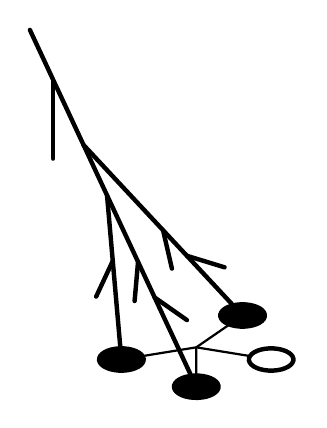
\begin{tikzpicture}
  [ draw/.append style={ultra thick,line cap=round},
    ground/.style={yscale=.5,rotate=-18,transform shape},
    station/.style={draw,circle,inner sep=.2cm},
    hit/.style={fill=black},
    datanet/.style={thick},
  ]
  \begin{scope}[ground]
    \coordinate (center) at (0,0) {};
    \foreach \i in {0,1,...,4} {
      \ifnum \i=2
      \else
        \ifnum \i=0
          \node[station] (station-\i) at (\i*360/5:1cm) {};
        \else
          \node[station,hit] (station-\i) at (\i*360/5:1cm) {};
        \fi
        \draw[datanet] (center) -- (station-\i);
      \fi
    }
  \end{scope}

  \coordinate (A) at ($ (station-4) + (115:5cm) $);
  \coordinate (B) at ($ (station-1) + (133:5cm) $);
  \coordinate (B') at (intersection of station-1--B and station-4--A);
  \coordinate (C) at ($ (station-3) + (95:5cm) $);
  \coordinate (C') at (intersection of station-3--C and station-4--A);
  \draw (station-4) -- (A);
  \draw (station-1) -- (B');
  \draw (station-3) -- (C');

  \coordinate (C1) at ($ (station-3)!.6!(C') $);
  \draw (C1) -- ($ (C1)!5mm!-30:(station-3) $);
  
  \coordinate (A1) at ($ (station-4)!.35!(A) $);
  \draw (A1) -- ($ (A1)!5mm!-30:(station-4) $);
  \coordinate (A2) at ($ (station-4)!.25!(A) $);
  \draw (A2) -- ($ (A2)!5mm!30:(station-4) $);
  
  \coordinate (B1) at ($ (station-1)!.5!(B') $);
  \draw (B1) -- ($ (B1)!5mm!-30:(station-1) $);
  \coordinate (B2) at ($ (station-1)!.35!(B') $);
  \draw (B2) -- ($ (B2)!5mm!30:(station-1) $);

  \coordinate (T) at ($ (A)!7mm!(station-4) $);
  \coordinate (T1) at ($ (T) + (0,-4.5mm) $);
  \coordinate (T1') at ($ (T1) + (10cm,0) $);
  \coordinate (T2) at ($ (T) + (0,-6mm) $);
  \coordinate (T3) at ($ (T) + (0,-10mm) $);
  \draw (T) -- (T3);
  %\draw (T1) -- (intersection of T1--T1' and A--station-4);
  %\node [base left=-1pt of T2] {\textsf{\Huge{HiSP}}};
  %\node [base right=6pt of T2] {\textsf{\Huge{RC}}};
\end{tikzpicture}

\end{document}